\section{Техническое задание}
\subsection{Основание для разработки}

Полное наименование системы: «Разработка интеллектуальной системы для выявления заболеваний сельскохозяйственных растений». Основанием для разработки программы является приказ ректора ЮЗГУ от «17» апреля 2025 г. № 1828-с приказа «О направлении (допуске) на практику». %«Об утверждении тем выпускных квалификационных работ».

\subsection{Цель и назначение разработки}

Программно-информационная система предназначена для диагностики заболеваний томатов по изображениям их листьев. Пользователями системы могут быть как агрономы, так и дачники.

Пользователи должны иметь возможность загружать фотографии поражённой листвы, получать результаты анализа и рекомендации по лечению и профилактике. Кроме того, система должна предоставлять краткое описание выявленного заболевания и возможные причины его возникновения.

Целью разработки является повышение эффективности сельскохозяйственного производства за счёт раннего выявления заболеваний и предоставления точных рекомендаций для их устранения. Это позволит сократить потери урожая, снизить затраты на химическую обработку и улучшить качество плодов.

Задачами данной разработки являются:
\begin{enumerate}
	\item Создание базы данных для хранения информации о заболеваниях, их симптомах, способах лечения и профилактики.
	\item Проектирование пользовательского интерфейса для удобной загрузки изображений и отображения результатов анализа.
	\item Разработка и обучение свёрточной нейросети для точной классификации заболеваний по изображениям.
\end{enumerate}

\subsection{Актуальность темы разработки}

Заболевания растений остаются одной из ключевых проблем в сельском хозяйстве. Они приводят к значительным потерям урожая и снижению его качества, поэтому крайне важной задачей является минимизация потерь за счёт внедрения современных технологий диагностики.

Разработка системы, основанной на использовании свёрточных нейронных сетей для распознавания заболеваний по фотографиям, актуальна по нескольким причинам. Во-первых, она позволяет сократить зависимость от квалификации специалистов, обеспечивая высокую точность диагностики даже для пользователей, которые не разбираются в агрономии. Во-вторых, такая система предоставляет возможность раннего выявления болезней, что существенно увеличивает шансы на успешное лечение. \cite{vkr3}

Кроме того, использование веб-технологий делает решение доступным для пользователей в любых регионах, где есть доступ к сети Интернет. Применение данного подхода может повысить эффективность сельскохозяйственного производства, сократить экономические потери и снизить экологическую нагрузку за счёт оптимизации использования химических средств защиты растений.

В сравнении с традиционными методами диагностики, предложенная система способна в течение нескольких секунд предоставить точный результат анализа, а воспользоваться ею можно везде, где есть Интернет. Эти факторы могут сделать данное решение удобным инструментом для современного сельского хозяйства.

\subsection{Этапы разработки}

Для реализации программной системы предполагается выполнение следующих этапов:
\begin{enumerate}
	\item Изучение существующих решений, определение перечня заболеваний томатов и их визуальных симптомов.
	\item Разработка структуры базы данных для хранения информации о заболеваниях, методах лечения и профилактики.
	\item Сбор и разметка набора данных, обучение модели YOLO 11 и её тестирование.
	\item Создание пользовательского интерфейса, интеграция CNN с веб-приложением.
	\item Проведение функционального тестирования, проверка точности диагностики.
\end{enumerate}

\subsection{Требования к программной системе}

\subsubsection{Требования к данным}
Входными данными для системы являются:
\begin{itemize}
	\item изображения листьев растений, которые пользователь загружает для анализа.
\end{itemize}
Выходными данными для системы являются:
\begin{itemize}
	\item информация о заболевании;
	\item данные об актуальных методах лечения и профилактики;
	\item сообщения об отсутствии информации о заболевании в базе.
\end{itemize}

\subsubsection{Функциональные требования}
Пользователю должны  быть доступны следующие функции:
\begin{itemize}
	\item загрузка фотографии пораженного листа томата для диагностики заболеваний;
	\item просмотр результатов анализа с информацией о выявленном заболевании;
	\item просмотр рекомендаций по лечению;
	\item просмотр информации по профилактике.
\end{itemize}
На рисунке ~\ref{diog1:image} представлена диаграмма прецедентов для пользователя.

\begin{figure}[H]
	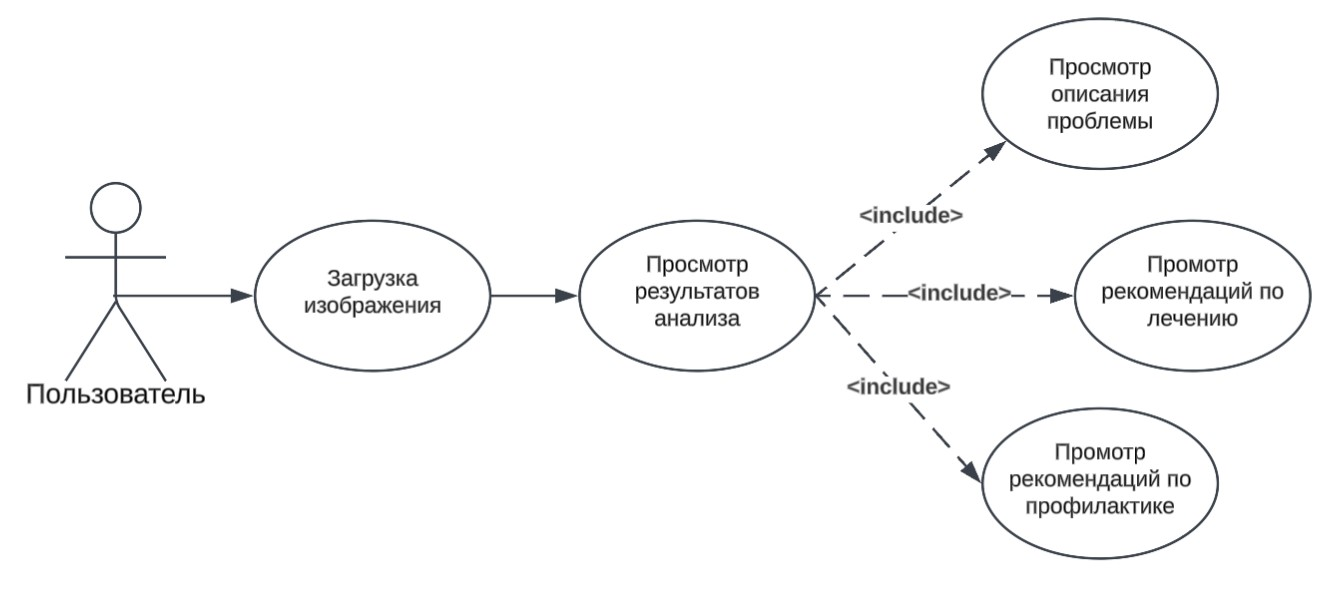
\includegraphics[width=1\linewidth]{diog1}
	\caption{Диаграмма прецедентов для пользователя}
	\label{diog1:image}
\end{figure}

\subsubsection{Сценарий прецедента пользователя «Загрузка изображения»}
Основной успешный сценарий:
\begin{itemize}
	\item пользователь заходит на главную страницу системы;
	\item выбирает опцию "Обзор...";
	\item выбирает изображение на своем устройстве;
	\item подтверждает выбор, нажав кнопку "Анализировать изображение";
	\item дожидается завершения анализа.
\end{itemize}

\subsubsection{Сценарий прецедента пользователя «Просмотр описания проблемы»}
Основной успешный сценарий:
\begin{itemize}
	\item изображение проанализировано;
	\item пользователь переходит к параграфу "Описание";
	\item просматривает информацию о найденной проблеме.
\end{itemize}

\subsubsection{Сценарий прецедента пользователя «Просмотр рекомендаций по лечению и профилактике»}
Основной успешный сценарий:
\begin{itemize}
	\item изображение проанализировано;
	\item пользователь переходит к параграфу "Лечение";
	\item просматривает способы устранить проблемы.
\end{itemize}

\subsubsection{Сценарий прецедента пользователя «Просмотр рекомендаций по профилактике»}
Основной успешный сценарий:
\begin{itemize}
	\item изображение проанализировано;
	\item пользователь переходит к параграфу "Профилактика".
	\item просматривает методы профилактики болезни.
\end{itemize}

\subsection{Требования пользователя к интерфейсу web-интерфейса}
Интерфейс должен быть интуитивно понятным, чтобы агрономы и обычные пользователи могли легко взаимодействовать с системой.
На рисунке ~\ref{maksite1:image} представлен макет страницы.

\begin{figure}[H]
	\centering
	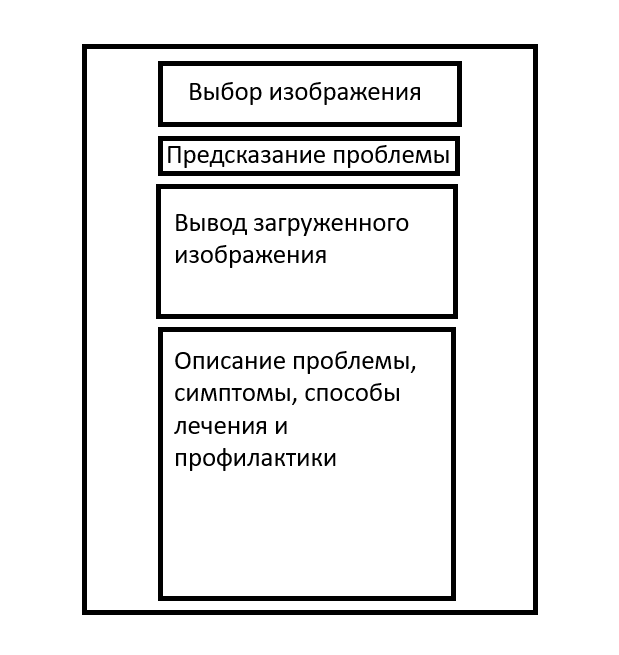
\includegraphics[width=0.9\linewidth]{макет изображения.png}
	\caption{Макет страницы}
	\label{maksite1:image}
\end{figure}

\subsection{Нефункциональные требования}

\subsubsection{Требования к программному обеспечению}

Для разработки и работы программной системы необходимы следующие компоненты:
\begin{itemize}
	\item среда разработки Python для реализации и настройки алгоритмов;
	\item фреймворк Flask для создания веб-приложения;
	\item СУБД PostgreSQL для хранения данных о пользователях, результатах анализа и рекомендациях;
	\item инструменты машинного обучения Ultralytics и Pytorch для работы с CNN;
	\item библиотеки OpenCV, PIL для обработки изображений и Pandas, NumPy для работы с данными.
\end{itemize}

Предлагаемые технологии поддерживаются на всех популярных операционных системах, таких как Windows, macOS и Linux \cite{python1}. Выбор таких инструментов обусловлен их гибкостью, производительностью и большим сообществом разработчиков, что упрощает разработку и последующую поддержку системы.

\subsection{Ограничения}

\begin{enumerate}
	\item Система ориентирована на диагностику заболеваний томатов и не поддерживает другие культуры, поэтому может выдавать ошибочные предположения при загрузке изображений других культур.
	\item Точность диагностики зависит от качества предоставленных входных данных.
	\item Для работы системы требуется стабильное интернет-соединение.
\end{enumerate}

\subsubsection{Требования к аппаратному обеспечению}
Для работы приложения требуется дисковое пространство не менее 2,5 Гб, минимум 2 Гб оперативной памяти и подключение к Интернету. Рекомендуется использовать процессор c 2 или более ядрами и частотой 2 ГГц или выше.

\subsection{Требования к оформлению документации}

Разработка программной документации и программного изделия должна производиться согласно ГОСТ 19.102-77 и ГОСТ 34.601-90. Единая система программной документации.
